% !TeX root = ../main.tex
% -*- coding: utf-8 -*-
% !TeX root = ../main.tex
% -*- coding: utf-8 -*-

\chapter{绪论}
\label{chpt:introduction}

链接预测的相关研究不仅有着重要的理论意义,能大力推动其它相关领域研究的进展,而且具有广泛的应用场景。
近年来,随着网络科学的快速发展,其理论上的成果为链接预测搭建了一个研究的平台,
使得链接预测的研究与网络的结构与演化紧密联系起来,
使得预测结果能从理论的角度上给出更合理的解释。
除此之外,链接预测的研究也可以从理论上帮助人们认识复杂网络的演化机制。
针对同一类网络,很多模型都提供了可能的网络演化机制\cite{吕琳媛2010复杂网络链路预测},
但描述网络拓扑结构的统计特征非常多,不仅很难比较哪个特征描述的更准确,
而且仅凭一两个特征往往很难从整体上刻画网络。
而链接预测机制有望为其提供一个简单统一且较为公平的比较平台,
从而大大推动复杂网络演化模型的理论研究。

\section{网络链接预测的背景}

在自然界和人类社会中广泛存在着各种各样的复杂系统,
这些复杂系统都可以用复杂网络的形式很好的表示出来。
网络中的点代表一个独立个体,
网络中的链接可代表个体间的关系或相互作用。
例如,互联网可以看作是由路由器或者接入Internet的计算机通过光纤等通信介质相互链接所形成的网络;
信息网络可以看作是信息的发送者和接收者之间通过信息传播路径所链接的关系网络;
生物体中的神经系统可以看作是大量的神经细胞通过神经纤维相互链接所形成的网络;
此外,还有社会关系网络、电力网络、科学家合作网络、蛋白质相互作用网络、交通网络等等。
因此,复杂网络的研究不仅对现实生活有非常重要的意义,对人类了解自然界和社会的发展也有着长远的科学指导意义,
而链接预测便是复杂网络研究中很重要的工作。\cite{刘宏鲲2011利用链路预测推断网络演化机制}

链接预测是通过利用网络的拓扑结构、节点属性等信息来预测网络内两个不相连的点是否会建立链接。
通常来说要预测的链接分为两种:一是已存在但未被发现的链接,二是未来可能产生建立的新链接\cite{李淑玲2012基于相似性的链接预测方法研究}\cite{wang2017novel}。


\section{链接预测的实际应用}
\subsection{链接预测在社交网络中的应用}
\label{intro:sec:social}
一个社交网络就是一个由社会中的个体以及这些个体间的关系构成的庞大社会结构。
可以把社交网络看作一个图,图中的节点表示社会中的个体,链接就表示个体间的关系或产生的交互\cite{李淑玲2012基于相似性的链接预测方法研究}。
目前,各类社交软件诸如微信、微博或Facebook等已逐渐成为人们日常生活中的一部分,
人们可借此平台方便的与他人分享信息,而由此也产生了一个庞大且复杂的社交网络,
且网络中海量的数据又有着质量高、数据量大、是现实社会关系的真实映射等很有价值的特点,
因此这些数据也吸引了来自不同领域的众多学者的目光\cite{wang2015link}。

\begin{figure}[h]
  \subfigure[Stanford 社交网络]{
    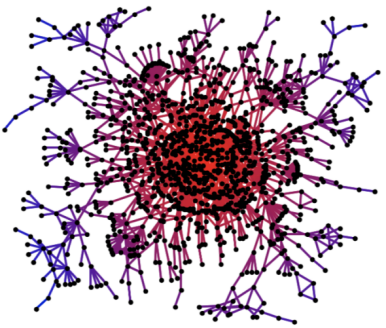
\includegraphics[]{stanford_social_net.png}
  }
  \subfigure[MIT 社交网络]{
  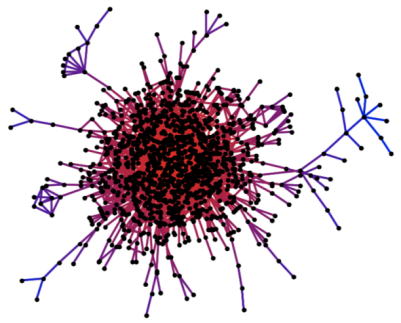
\includegraphics[]{MIT_social_net.png}
  }
  \caption{社交网络示意}
  \label{intro:fig:social_net}
\end{figure}
Lada A. Adamic 和Eytan Adar在2003年通过分析大学中学生的个人主页构建出了一个小型社交关系网络\cite{adamic2003friends}。
他们观察到,学生经常会在自己的个人主页中提及自己的朋友,
而这主要是通过使用超链接指向对方的个人主页或在朋友列表中列出对方的邮件地址;
此外,个人主页中的某些文本也可以用来揭示社交关系,例如有两个人在自己的主页中都提到了“机器学习”这门课程,
那么这两人便有可能因为在同一间教室上课而成为朋友。
作者分别使用MIT和斯坦福大学中的个人主页成功构建出了两个社交网络,
其中每个学生作为一个节点,节点间的链接是通过分析了上述几个信息源后标注出的。
图\ref{intro:fig:social_net} 展示了两所大学内的社交网络。


\begin{center}
\tablecaption{对Chao.C.H的预测结果}
\begin{tabular}{c|c|c}\hline
\multicolumn{3}{c}{CAnakken: Clifford Hsiang Chao}\\ \hline
是否为朋友 & 相似度 & 姓名\\ \hline
否 & 8.25 & Eric Winston Liao\\
是 & 3.96 & John Andrew Vestal\\
否 & 3.27 & Desiree Dawn Ong \\
是 & 2.82 & Stanley Hsinheng Lin\\
否 & 2.66 & Daniel Sunil Chai \\
否 & 2.55 & Wei Nan Hsu \\
是 & 2.42 & David J.Lee \\
否 & 2.41 & Hands Christian Andersen \\
否 & 2.41 & Byung Joo Lee\\ \hline
\label{intro:table:chao}
\end{tabular}
\end{center}


为了预测某两人是否为朋友,文中对每两个人之间的相似度做了排序然后直观的给出结论:
两个人间相似度越高就越可能是朋友。在定义了合适的相似度计算方式后便得到了所有人互相成为朋友的概率。
表\ref{intro:table:chao} 以名为Clifford Hsiang Chao的学生为例给出了他与前九名相似度最高的学生的真实关系,
从中可以看出,算法在保证了一定准确率的同时也提供了潜在的可能成为朋友的人。

\subsection{链接预测在医学中的应用}
链接预测在医学界的一个典型应用就是对药物-药物相互作用(Drug-Drug Interaction, DDI)的预测。
DDI是导致药物潜在危害反应的一个重要原因,尤其是在当病人同时摄入多种药物的时候\cite{fokoue2016predicting}。
例如最近的研究显示,老年人是最常见的同时摄入多种药物的群体,并且大约在每25人中就会有一个人受到过因DDI产生的危害\cite{huang2013systematic}\cite{juurlink2003drug}。
再比如用于临床治疗患有情绪障碍(如重度抑郁症)的患者时常使用的三环类抗抑郁药物也被认为会经常引起药物间反应,
一是由于这类患者往往患有其它伴随病症从而需要服用多种其它药物,二是情绪障碍类疾病的治疗周期很长,
即需要长时间服用药物。如今的许多处方药,如“拜新同”(一种降压药),都会在其药品说明书中列出与其它类药物共同使用时可能发生的反应。

因此,发现和预测DDI不仅可以预防临床用药时发生的不良反应,还可以帮助开出含有共同药物的处方以提供更好的治疗效果\cite{zhang2018prioritizing}。
虽然前人已经做了很多努力去寻找可能的DDI并将已知信息存入到了数据库中,如:KEGG、DrugBank以及STITCH。
但最近的研究显示,没有一种数据源能涵盖所有的DDI,而且大部分的数据源要么不完整要么就是保守地列出了许多“无关痛痒”的DDI\cite{fokoue2016predicting}。
而近些年出现的一个新研究方向是基于药物本身的机制、结构信息或与蛋白质的相互作用来预测新型DDI。
预测方法类似于在研究社交网络时使用的计算相似性的方法。\cite{vilar2012drug}通过计算药物间分子结构的相似性来预测DDI,其基于的假设就是,
如果药物A与药物B具有相似的分子结构,则那些会与A发生有害反应的药物也很有可能与B也产生相似反应。
举例来说,据Medical Literature研究显示,辛伐他汀是一种通过抑制HMG-CoA还原酶来降低胆固醇水平的药物,
可以与三唑类抗真菌药物氟康唑相互作用,导致肌病或横纹肌溶解症的风险增加;则根据文中的假设,
那些类似于辛伐他汀的药物也可以与氟康唑相互作用并产生如上所述的类似的相互作用。
图\ref{intro:fig:process}以此为例展示了主要的计算过程。

\begin{figure} 
  \centering
  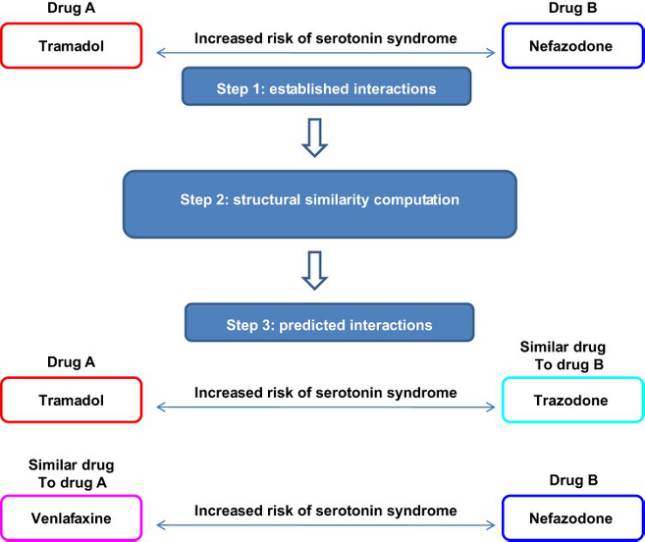
\includegraphics[width=8cm, height=8cm]{example_predict_process.png}
  \caption{以分子结构作为相似度的计算过程\cite{vilar2012drug}}
  \label{intro:fig:process}
\end{figure} 

图\ref{intro:fig:result}举例列出了算法在2009年售出最多的50种药中预测出的相互作用,它们尚未被DrugBank验证。

\begin{figure} 
  \centering
  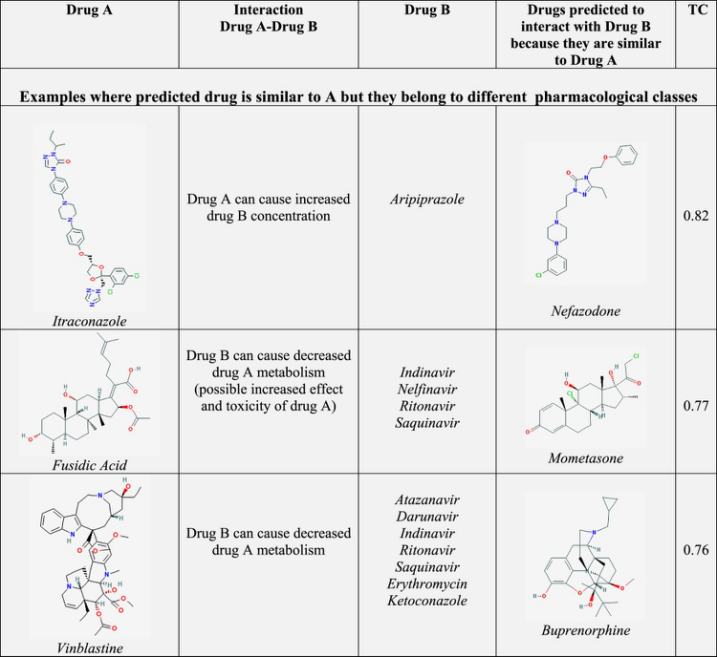
\includegraphics[width=8cm,height=9cm]{example_predict_result.png}
  \caption{对实际药物的预测结果举例\cite{vilar2012drug}}
  \label{intro:fig:result}
\end{figure} 

\subsection{链接预测在其他领域中的应用}
除上述两个典型场景外,链接预测算法也在其他领域有着广泛的应用:
在电子商务中链接预测可以用来构建推荐系统;
在图书馆科学中,可以利用链接预测来删除重复数据;
在信息检索领域中,为提高检索效率,可以利用链接预测技术改进搜索引擎和信息检索的超文本分析\cite{李淑玲2012基于相似性的链接预测方法研究};
除此之外链接预测还可以用来判断学术论文的类型、判断手机用户是否产生了切换运营商的念头\cite{李淑玲2012基于相似性的链接预测方法研究}或者重新规划航班线路。


\section{国内外研究现状}
\label{intro:sec:study}
目前的链接预测算法主要分为三类:基于相似度的、基于路径的和基于矩阵分解的方法\cite{lu2009similarity}。本节将简单介绍各类别方法中的一些经典算法。

\subsection{基于相似度的方法}
在所有基于相似度的算法中,
Common Neighbors(CN)算法和\ref{intro:sec:social} 节提到的Adamic-Adar(AA)算法可谓最具代表性的两个算法。
前者将节点间相似度定义为两节点间共同邻居(即相同邻接点)的个数;
后者在这之上对邻接点的度数做了惩罚以减弱“富人俱乐部”效应,两个算法都成功做出了链接预测。
在这之后,许多基于这两个方法的新算法如雨后春笋般被提出来,它们要么是在原算法的基础上做了改动,要么是使用了CN或AA的结果作为相似度的依据之一。


陈槿慧等人在2015年使用信息论的方法提出了一个基于共同邻居集合的算法,叫做NSI。
该算法在面对具有多重结构特征的数据时很有效。NSI从信息论的角度衡量了网络中拓扑结构的特点,不同的拓扑结构含有不同的隐含信息并进而影响到对链接的预测\cite{chen2014robust}。


Scellato等人在药物-药物关联预测领域提出了一个网络连通性指标(network-connectivity score)来衡量药物和对应靶蛋白间关系的强弱。
略具体来说,算法使用了三种数据:药物-药物关联数据、药物-蛋白关联数据以及蛋白-蛋白关联数据,
然后算法利用药物-蛋白关联数据将药物映射到了蛋白网络中,通过对蛋白网络中药物相关节点集的系统连通性进行评分,计算目标网络中节点对的相似度\cite{scellato2011exploiting}。


\subsection{基于路径的方法}
基于路径的链接预测算法更多关注网络的拓扑结构信息,Katz提出了一个经典算法来计算节点对之间所有的潜在路径,
其损失函数中对路径长度做了惩罚,即越长的联通路径损失越大\cite{elhamifar2013sparse}。


张平等人提出了一个称为LP的标签传播算法\cite{zhang2015label},该算法将相似性的使用分为一阶和二阶来链接具有相同标签的节点。
除了用于目标网络的标签传播算法之外,损失函数由从不同辅助信息导出的各个相似性矩阵线性组合。


徐中启等人用信息论的方法量化了节点路径特点对链接预测的影响并以此提出了一个用于预测用户社交关系的算法。
算法通过引入辅助数据“用户对不同地理位置的到访记录”,计算出了一个路径熵(Path Entropy)指标,依此做链接预测\cite{xu2016link}。

\subsection{基于矩阵分解的方法}
Menon等人提出使用监督矩阵分解方法解决图中的链接预测问题,
他们综合考虑了(从目标网络中分解得到的)隐含特征、节点本身的特征以及链接的特征,算法使用了随机梯度下降的方法优化\cite{singh2008relational}。


Singh等人为进一步提升预测准确率而综合考虑了数据中的多种关系,将其统一后给出了新的矩阵分解公式,
当对由不同关系形成的多个矩阵进行分解时,不同元素的系数会根据情况来“共享”。


曹珠等人将矩阵补全和子图嵌入思想结合起来进行表征学习。其中,子图嵌入用于捕获细粒度的节点特征,凸矩阵补全用于去除噪声和迭代地提高泛化能力\cite{cao2018link}。


Guimerà等人提出了一种称为MCLP的替代迭代算法来解决矩阵补全问题,目标网络被视为缺失的数据集,并通过矩阵补全从拓扑结构信息中恢复潜在的链接\cite{guimera2009missing}。

\section{论文组织结构}
本论文一共分为四章,其中二、三章为论文主体部分,各章内容分别为:


第一章为绪论,主要介绍了链接预测问题的背景、举例介绍了相关算法在实际问题中的应用然后简要分析了国内外在该领域的研究进展。


第二章介绍算法,提出了协同线性流形学习算法并给出各部分的推导过程。


第三章为实验部分,首先介绍了实验所用的数据来源,简单分析了数据集的结构特点,介绍了实验常用的评价指标,然后详细介绍了引入的一系列实验并分别做了实验分析。


总结了算法的性能并展望了今后工作中可能的着手点。